\vspace{-0.3in}
\begin{abstract}
\vspace{-0.05in}
	Multi-task learning is a powerful approach in many applications such as image and text classification. Yet, there is little rigorous understanding of when multi-task learning outperforms single-task learning. In this work, we provide a rigorous study to anwer the question in the high-dimensional linear regression setting. We show that the bias-variance tradeoff of multi-task learning determines the effect of information transfer and develop new concentration bounds to analyze the tradeoff. Our key observation is that three properties of task data, namely \textit{task similarity}, \textit{sample size}, and \textit{covariate shift} can affect transfer in the high-dimensional linear regression setting. We relate each property to the bias and variance of multi-task learning and explain three negative effects with decreased task similarity,	increased source sample size, and covariate shift under increased source sample size. And we validate the three effects on text classification tasks. Inspired by our theory, we show two practical connections of interest.
	First, single-task performance can help understand multi-task performance.
	Second, incrementally adding training data can mitigate negative transfer and improve multi-task training efficiency.
\end{abstract}

\vspace{-0.15in}
\section{Introduction}

%Multi-task learning is an inductive learning mechanism to improve generalization performance using related task data.
%Many state-of-the-art results in computer vision and natural language processing are obtained using multi-task learning.
Multi-task learning is a powerful approach for improving performance on many tasks in computer vision \cite{chexnet17,ZSSGM18}, natural language processing \cite{GLUE,superglue}, and other areas \cite{ZY17}.
%In multi-task learning, having related task data is fundamental to its performance.
%Multi-task learning is particularly powerful when there is limited labeled data for a task to be solved, meanwhile more labeled data from different but related tasks is available.
%By combining multiple information sources, it is possible to share all the information in the same model.
In many settings, multiple source tasks are available to help predict a particular target task.
%For example, many applications in , and many other areas have been achieved by learning from multiple tasks together.
The performance of multi-task learning depends on the relationship between the source and target tasks \cite{C97}.
%	We define that multi-task learning provides \textit{positive transfer} if it outperforms single-task learning, or \textit{negative transfer} otherwise.
When the sources are relatively different from the target, multi-task learning has often been observed to perform worse than single-task learning \cite{AP16,BS17}, which is referred to as \textit{negative transfer} \cite{PY09}.
While many empirical approaches have been proposed to mitigate negative transfer \cite{ZY17}, a precise understanding of when negative transfer occurs remains elusive in the literature \cite{R17}.
%This phenomenon, known as \textit{negative transfer}, is fundamental to the understanding of multi-task learning.

%Inspired by the theory, we propose an incremental training schedule to improve multi-task training.
%We consider a setting where the target task has limited labeled data and show
%On the other hand, unless the structures across task data are well-understood, applying multi-task learning on several different datasets often result in suboptimal models (or negative transfer in more technical terms).

However, understanding negative transfer requires developing generalization bounds that scale tightly with properties of each task data such as its sample size.
This presents a technical challenge in the multi-task setting because of the difference among task features, even for two tasks.
For Rademacher complexity or VC-based techniques, the generalization error scales down as the sample sizes of all tasks increase, when applied to the multi-task setting \cite{B00,AZ05,M06,MPR16,WZR20}.
Without a tight lower bound for multi-task learning, comparing its performance to single-task learning results in vacuous bounds.
From a practical standpoint, developing a better understanding of multi-task learning in terms of properties of task data can provide guidance for downstream applications \cite{RH19}.
%For example, the sample sizes of all tasks are often assumed to be equal \cite{B00,LPTV09,LPVT11}.
%On the other hand, uneven sample sizes (or dominating tasks) have been empirically observed to cause negative transfer \cite{YKGLHF20}.
%The benefit of learning multi-task representations has also been studied for certain half-spaces \cite{} and sparse regression \cite{}.
%When all tasks are sufficiently similar, adding more labeled data improves the generalization performance for predicting a particular task \cite{WZR20}.

%\textbf{Setup and Main Results.}
In this work, we study the bias and variance of multi-task learning in the high-dimensional linear regression setting \cite{HMRT19,BLLT20}.
Our key observation is that three properties of task data, including \textit{task similarity}, \textit{sample size}, and \textit{covariate shift} can affect whether multi-task learning outperforms single-task learning (which we refer to as \textit{positive transfer}).
As an example, we vary each property in Figure \ref{fig_model_shift_phasetrans} for two linear regression tasks and measure the improvement of multi-task learning over single-task learning for task two.
We observe that the effect of transfer can be positive or negative as we vary each property.
These phenomena cannot be explained using previous techniques \cite{WZR20}.
The high-dimensional linear regression setting allows us to measure the three properties precisely.
We define each property for the case of two tasks and our definition applies to general settings.
We refer to the first task as the source task and the second as the target task.
\squishlist
	\item \textbf{Task similarity:} Assume that both tasks follow a linear model with parameters $\beta_1, \beta_2\in\real^p$, respectively.
	We measure the distance between them by $\norm{\beta_1 - \beta_2}$.
	\item \textbf{Sample size:} Let $n_1 = \rho_1 \cdot p, n_2 = \rho_2 \cdot p$ be the sample size of each task, where $\rho_1, \rho_2>1$ are both fixed values that do not grow with $p$.
	We measure the source/target sample ratio by $\rho_1 / \rho_2$.
%	Importantly, $\rho_2$ can be a small constant (say $2$) to capture the need for more labeled data.
	\item \textbf{Covariate shift:} Assume that the task features are random vectors with positive semidefinite covariance matrix $\Sigma_1,\Sigma_2\in\real^{p\times p}$, respectively.
	%$x = \Sigma_i^{1/2}z$, where $z\in\real^p$ consists of i.i.d. entries with mean zero and unit variance, and is a positive semidefinite matrix.
	We define covariate shift as the matrix $\Sigma_1^{1/2}\Sigma_2^{-1/2}$.
\squishend

%The observations highlight the need to develop generalization bounds that scale tightly with properties of multiple tasks data.
% that only contains limited amount of labeled data.
%Following Hastie et al.  and Bartlett et al. \cite{},

%Let $n_i = \rho_i \cdot p$ denote the data size and $X_i\in\real^{n_i\times p}$ denote the features of task $i$.
%The labels of task $i$ are given by $Y_i = X_i\beta_i + \varepsilon_i$, where $\beta_i\in\real^p$ denotes task $i$'s ground truth parameters and $\varepsilon_i$ denotes i.i.d. random noise with mean zero and variance $\sigma^2$.
We consider a multi-task estimator obtained using a shared linear layer for all tasks and a separate output layer for each task \cite{WZR20}.
This two-layer model is inspired by a commonly used idea of hard parameter sharing in multi-task learning \cite{R17,MTDNN19}.
We consider the bias and variance of the multi-task estimator for predicting a target task and compare its performance to single-task learning.
%This corresponds to minimizing $ \sum_{i=1}^t \norm{X_i B W_i - Y_i}^2$.
%Let $\hat{\beta}_t^{\MTL}$ denote the optimal multi-task estimator for the target task, which is defined precisely in Section \ref{sec_prelim}.
%We revisit the bias-variance tradeoff of $\hat{\beta}_t^{\MTL}$.

\textbf{Main results.} First, we develop tight bounds for the bias and variance of the multi-task estimator for two tasks by applying recent development in random matrix theory \cite{erdos2017dynamical,isotropic,Anisotropic}.
We observe that the variance of the multi-task estimator is \textit{always smaller} than single-task learning, because of added source task samples.
On the other hand, the bias of the multi-task estimator is \textit{always larger} than single-task learning, because of model differences.
Hence, the tradeoff between bias and variance determines whether the transfer is positive or negative.
We provide a sharp analysis of the \textit{variance} that scales with sample size and covariate shift.
We extend the analysis to the bias, which \textit{in addition} scales with {task similarity}.
Combining both, we analyze the bias-variance tradeoff for two tasks in Theorem \ref{thm_main_informal} and extend the analysis to many tasks with the same features in Theorem \ref{thm_many_tasks}.
%For the setting of two tasks, we show how the variance of the multi-task estimator  scales with sample size and covariate shift in the following result.
%\textit{Our first contribution} is to develop a concentration bound that arises naturally from the bias-variance tradeoff of $\hat{\beta}_t^{\MTL}$ for two tasks.
%Let $\hat{\beta}_t^{\STL}$ denote the single-task estimator.
%Without loss of generality, let the $t$-th task denote the target task.
%Importantly, the target task's data size is a fixed constant times $p$ in the high-dimensional setting.
%Hence adding more labeled data can help improve its test performance.
%$B\in\real^{p\times r}$
%$\set{W_i \in \real^{r}}_{i=1}^t$

\begin{figure}[!t]
	\begin{subfigure}[b]{0.32\textwidth}
		\centering
		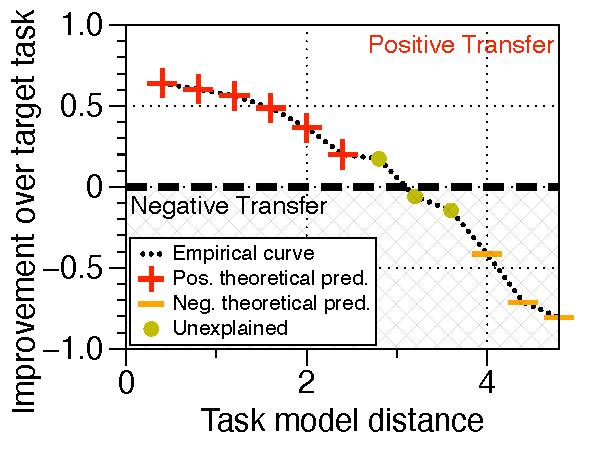
\includegraphics[width=0.98\textwidth]{figures/model_shift_phase_transition.pdf}
		\vspace{-0.075in}
		\caption{Task similarity}
		\label{fig_model_shift}
	\end{subfigure}\hfill
	\begin{subfigure}[b]{0.32\textwidth}
		\centering
		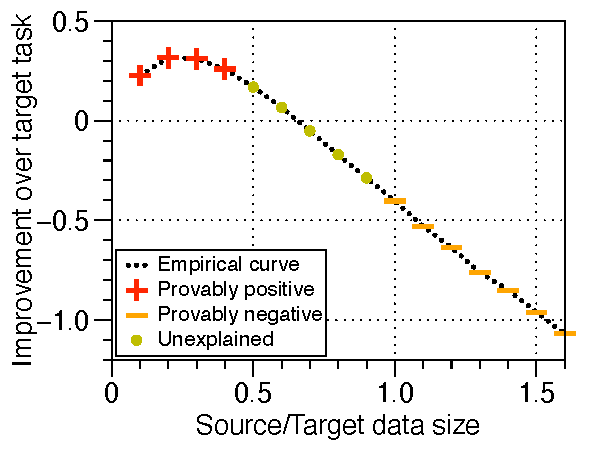
\includegraphics[width=0.98\textwidth]{figures/datapoints_phase_transition.pdf}
		\vspace{-0.075in}
		\caption{Sample size}
		\label{fig_size}
	\end{subfigure}\hfill
	\begin{subfigure}[b]{0.32\textwidth}
		\centering
		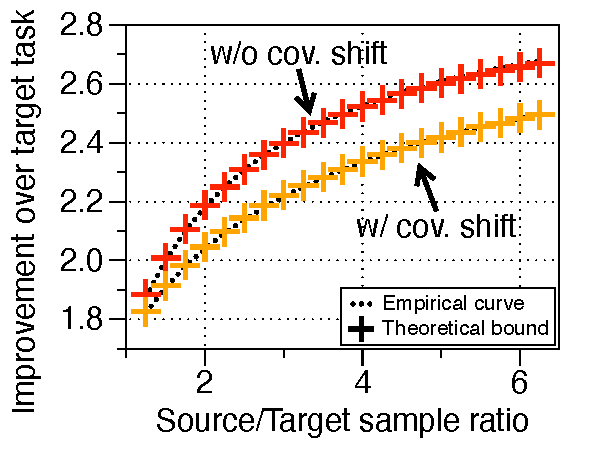
\includegraphics[width=0.98\textwidth]{figures/complementary.pdf}
		\vspace{-0.075in}
		\caption{Covariate shift}
		\label{fig_covariate}
	\end{subfigure}
	\caption{%Three takeaways of our theory in Section \ref{sec_insight}.
	We observe a transition from positive to negative transfer as (a) \textit{task model distance} increases and (b) source/target \textit{sample ratio} increases.
	For the special case of having the same task model, we observe in (c) that as source/target \textit{sample ratio} increases, having \textit{covariate shift} worsens the performance of MTL.
	The $y$-axis measures the loss of STL minus MTL.}
	\label{fig_model_shift_phasetrans}
	\vspace{-0.3in}
\end{figure}


%Concretely, we show a tight bound on the trace of $(X_1^{\top}X_1 + X_2^{\top}X_2)^{-1}$, which
%Theorem \ref{lem_cov_shift_informal} allows us to analyze the bias-variance tradeoff of the multi-task estimator for two settings:
%(i) two tasks with arbitrary covariate shift; (ii) many tasks with no covariate shift.

%We shall assume that each task data follows a linear model, i.e. $y_i = X_i \beta_i + \varepsilon_i$, $1\le i\le k$.
%Here $\beta_i\in\real^p$ is the model parameter for the $i$-th task.
%Each row of $X_i\in\real^{n_i\times p}$ is assumed to be drawn i.i.d. from a fixed
%distribution with covariance matrix $\Sigma_i$.

%We extend our result to the transfer learning
%in the setting of high-dimensional linear regression.
%by pooling source task representations into the shared body of the hard parameter sharing architecture, following
%setting of Taskonomy by Zamir et al. \cite{ZSSGM18}.
%We prove that the bias of the transfer learning estimator is given by the projection of $\beta_t$ to the orthogonal subspace spanned by $\set{\beta_i}_{i=1}^{t-1}$.
%These results are described more precisely in Section \ref{sec_main}.

Second, we explain the phenomena in Figure \ref{fig_model_shift_phasetrans} in isotropic and covariate shifted settings.
%We observe that negative transfer occurs as (a) \textit{task similarity}: tasks become more different; (b) \textit{data size}: source/target data size increases.
%\textbf{Task similarity:}
%\textbf{Data sizes:}
%\textbf{Covariate shift:}
%Furthermore, MTL performance is negatively affected when (c) \textit{covariate shift}: the covariance matrices of the two tasks become more different.
\squishlist
	\item We provide conditions to predict the effect of transfer as a parameter of model distance $\norm{\beta_1-\beta_2}$ (Section \ref{sec_similarity}).
	As model distance increases, the bias becomes larger, resulting in negative transfer.
%	Our result predicts most of the empirical observations in Figure \ref{fig_model_shift} correctly.
%	It is crucial that the concentration result in Theorem \ref{lem_cov_shift_informal} is sufficiently precise so that we can explain the transition phenomena in Figure \ref{fig_model_shift} and \ref{fig_size}.
%	The unexplained observations are caused by an error term from the bias.
%	We discuss these in Section \ref{sec_insight}.
	\item We provide conditions to predict transfer as a parameter of sample ratio $n_1/n_2$ (Section \ref{sec_data_size}).
	Adding source task samples helps initially by reducing variance, but hurts eventually due to bias.
	%namely adding more labeled data from the source task does not always improve performance (Proposition \ref{prop_data_size}).
	%Theorem \ref{lem_cov_shift_informal} allows us to compare MTL performance under different covariate shifts.
	\item For a special case of $\beta_1=\beta_2$, we show that MTL performs best when the singular values of $\Sigma_1^{1/2}\Sigma_2^{-1/2}$ are the same  (Section \ref{sec_covshift}).
	Otherwise, the variance reduces less with covariate shift.
%	Our theoretical bound matches the empirical curve in Figure \ref{fig_covariate}.
\squishend
%In Section \ref{sec_insight}, we consider three components including task similarity, data size and covariate shift for a simplified isotropic setting of two tasks.
%We measure task similarity by how small is the distance between $\beta_1$ and $\beta_2$.
%Using our tool, we explain a transition from positive to negative transfer as task similarity decreases.
%		Furthermore, we show that negative transfer is more likely to occur when the source task labels are particularly noisy.
%		In Section \ref{sec_validate}, we validate the observation on text and image classification tasks.
%	In , we provide the trade-off between $\norm{\beta_1 - \beta_2}^2$ and a certain function $\Phi(\rho_1, \rho_2)$ to determine the type of transfer.
%We show that increasing the data size of the source task does not always improve performance for the target task in multi-task learning.
Along the way, we analyze the benefit of MTL for reducing labeled data to achieve comparable performance to STL, which has been empirically observed in Taskonomy by Zamir et al. \cite{ZSSGM18}.
%We show that covariate shift, measured by $\Sigma_1^{1/2}\Sigma_2^{-1/2}$, is another cause for suboptimal performance for $\hat{\beta}_t^{\MTL}$.
%		We show that as $n_1 / n_2$ becomes large, having no covariate shift between the source and target tasks yields the optimal performance for the target task.
%		On the other hand, when $n_1 / n_2$ is small, there are counter examples where having the same covariance matrix is not necessarily the optimal choice.

Our study also leads to several algorithmic consequences with practical interest.
First, we show that single-task learning results can help predict positive or negative transfer for multi-task learning.
We validate this observation on ChestX-ray14 \cite{chexnet17} and sentiment analysis datasets \cite{LZWDA18}.
Second, we propose a new multi-task training schedule by incrementally adding task data batches to the training procedure.
This is inspired by our observation in Figure \ref{fig_size} where adding more source task data helps initially, but hurts eventually.
Using our incremental training schedule, we reduce the computational cost by $65\%$ compared to baseline multi-task training over six sentiment analysis dataset while keeping the accuracy the same.
Third, we provide a fine-grained insight on a covariance alignment procedure proposed in \cite{WZR20}.
We show that the alignment procedure provides more significant improvement when the source/target sample ratio is large.
Finally, we validate our three theoretical findings on sentiment analysis tasks.
